\documentclass[14 pt, fleqn, pstricks]{extarticle}

	\usepackage[frenchb]{babel}
	\usepackage[utf8]{inputenc}  
	\usepackage[T1]{fontenc}
	\usepackage{amssymb}
	\usepackage[mathscr]{euscript}
	\usepackage{stmaryrd}
	\usepackage{amsmath}
	\usepackage{tikz}
	\usepackage[all,cmtip]{xy}
	\usepackage{amsthm}
	\usepackage{varioref}
	\usepackage{geometry}
	\usepackage{tabularx}
	\geometry{a4paper}
	\usepackage{lmodern}
	\usepackage{hyperref}
	\usepackage{array}
	 \usepackage{fancyhdr}
	 \usepackage{pstricks,pst-plot,pst-tree,pstricks-add}
\usepackage{pst-eucl}% permet de faire des dessins de géométrie simplement
\usepackage{pst-text}
\usepackage{pst-node,pst-all}
\usepackage{pst-func,pst-math,pst-bspline,pst-3dplot}  %%% POUR LE BAC %%%
	 \usepackage{float}\usepackage{setspace}
\setlength{\mathindent}{1cm}
\renewcommand{\theenumi}{\alph{enumi})}
	\pagestyle{fancy}
	\theoremstyle{plain}
	\fancyfoot[C]{} 
	\fancyhead[L]{}
	\fancyhead[R]{}\geometry{
 a4paper,
 total={170mm,257mm}
 }
	
	
	\title{Exercices de calcul}
	\date{}
	\begin{document}
	 


\subsection*{Exercice 1 (6 points) }	 
	 
	 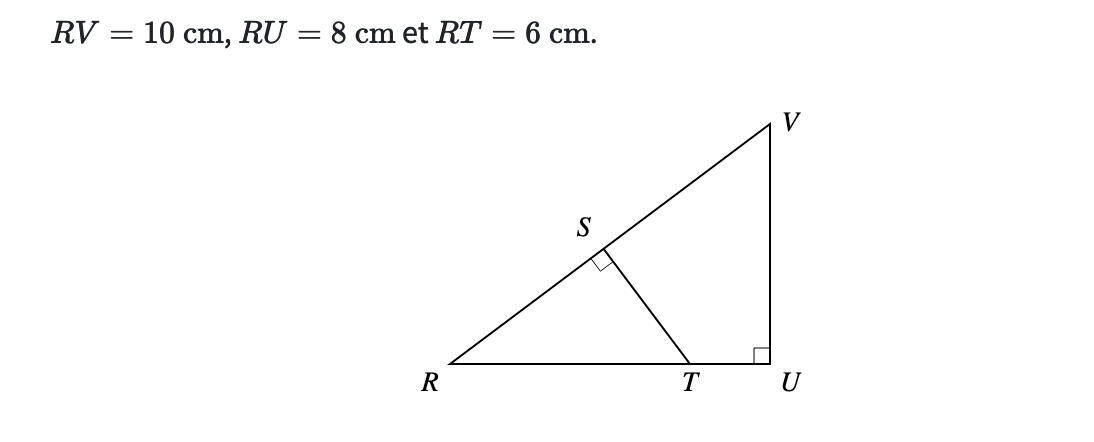
\includegraphics[width=18 cm]{Exo1}
\begin{enumerate}
\item Calculer l'angle $\widehat{SRT}$. 
\item En déduire la longueur $RS$, et donner une valeur approchée au millimètre près. 
\item Les triangles $RST$ et $RUV$ sont-ils semblables ?
\end{enumerate}
\subsection*{Exercice 2 (8 points)}

Résoudre les équations suivantes en laissant vos étapes : 
\begin{enumerate}
\item $2x + 1 = 9$ 
\item $ \frac{5 x - 1}2 = 12$. 
\item $ 9 x + 4  = 8 x - 23$
\item $ 3x + 1 = -8 x +122$ 
\end{enumerate}

\subsection*{Exercice 3 (6 points)}
Une certaine somme est partagée entre $3$ personnes. La première en reçoit le tiers, la seconde les quatre neuvièmes moins 1360 euros, et la dernière les deux septièmes moins 2120 euros. 
\begin{enumerate}
\item Exprimer chacun des lots en fonction de la somme totale $x$. 
\item En déduire une équation sur $x$. 
\item La résoudre, et en déduire ce que reçoit chaque personne. 
\end{enumerate}
 	\end{document}







